% !TeX root = thesis.tex
\documentclass{master_thesis}
\addbibresource{refs.bib}

\begin{document}

\section{Results}

\todo{Follow up survey + reach out to devs I know have used addon-a11y}
\todo{This section should have answers to all my research questions}
\todo{Limitations of manual testing - resources, we only had this many people to perform the review}
\todo{Come up with a list of things that should be tested manually, based on my case study}


\subsection{Comparing results from manual audit and automated report}

To get the whole list including all components, a report was created that included the violations caught in each example of each component. This report was generated at the beginning of the manual audit, so the results obtained from both methods are based on the same source code. A comparison table from both results was compiled. This included \textit{unique violations detected for component}, \textit{report\_violations}, \textit{violations}, \textit{true\_violations}, \textit{passes detected for component}, \textit{passes}, \textit{true\_passes}, and \textit{explanation of false violations and passes} and the summarized results from manual testing \textit{violations from manual testing for component}, \textit{manual\_count}. These are explained in more detail in chapter \ref{adding-a11y-tool}: \nameref{adding-a11y-tool}. Based on this synthesized data a comprehensive analysis of the results could be carried out.

Addon-a11y did not report any violations for 27 (51\%) components out of 53 components after verifying the validity of these issues the number goes up to 31 (58\%) (see Figure \ref{fig:audit-failed}). On average the automated testing tool found 1 violation per component. The maximum number of violations reported for a single component was 7 and the maximum number of valid violations was 6.

4 components out of 53 did not have any passed checks and 22 did not have any valid passed checks (see figure \ref{fig:audit-passed}). This means that the number of components with no valid passed checks changed from 4\%  to 42\% after manually validating the results. The highest number of passes were detected for Form and Table component (18). After validating the number of passes changed to 9 for Table and 7 for Form. The average number of passes for each component was 5 before and 2 after validating the results.

\begin{figure}[ht]
	\begin{subfigure}{0.45\textwidth}
	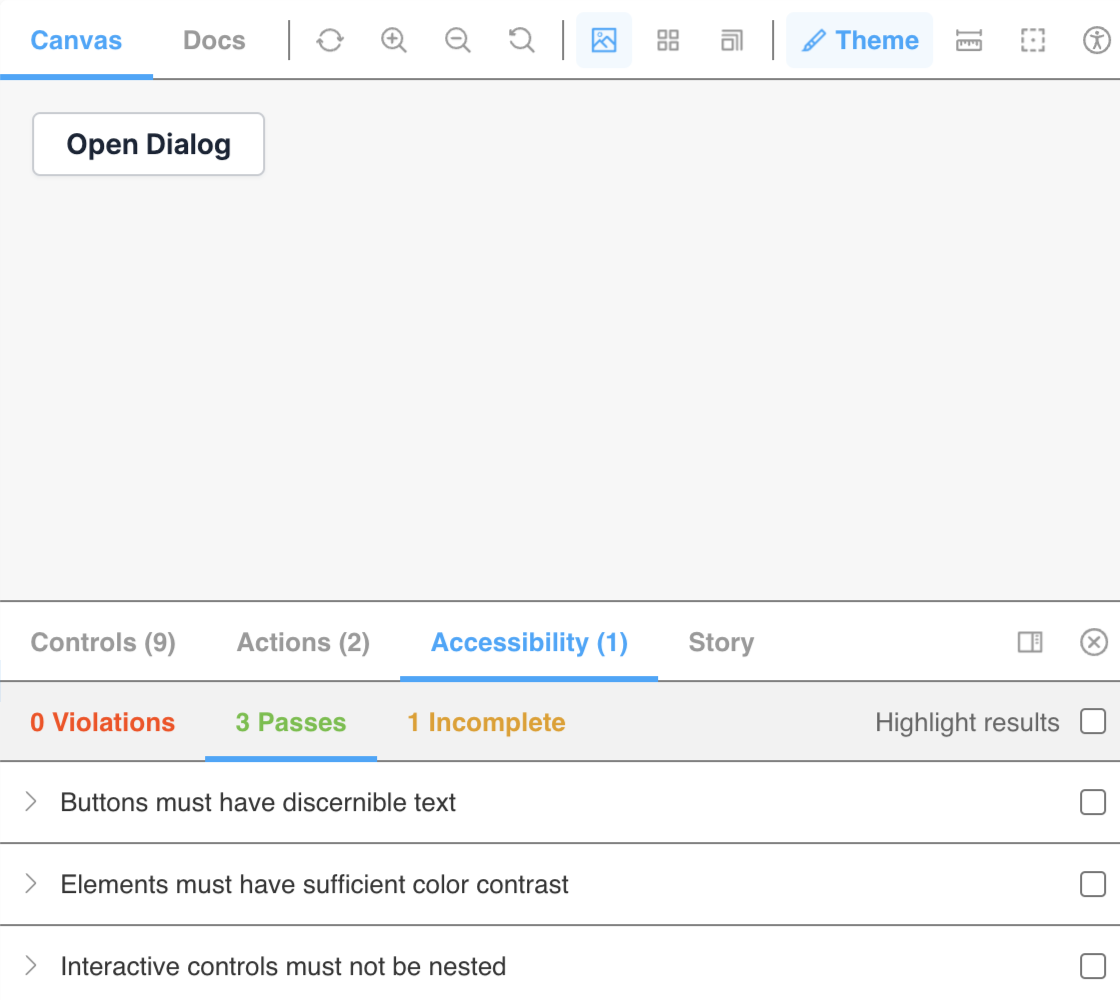
\includegraphics[width=\textwidth]{img/sb-button-trigger.png}
	\caption{Inital view of example. This is tested by addon-a11y.}
	\label{fig:sb-button-trigger-1}
	\end{subfigure}
	\hspace{0.05\textwidth}
	\begin{subfigure}{0.45\textwidth}
	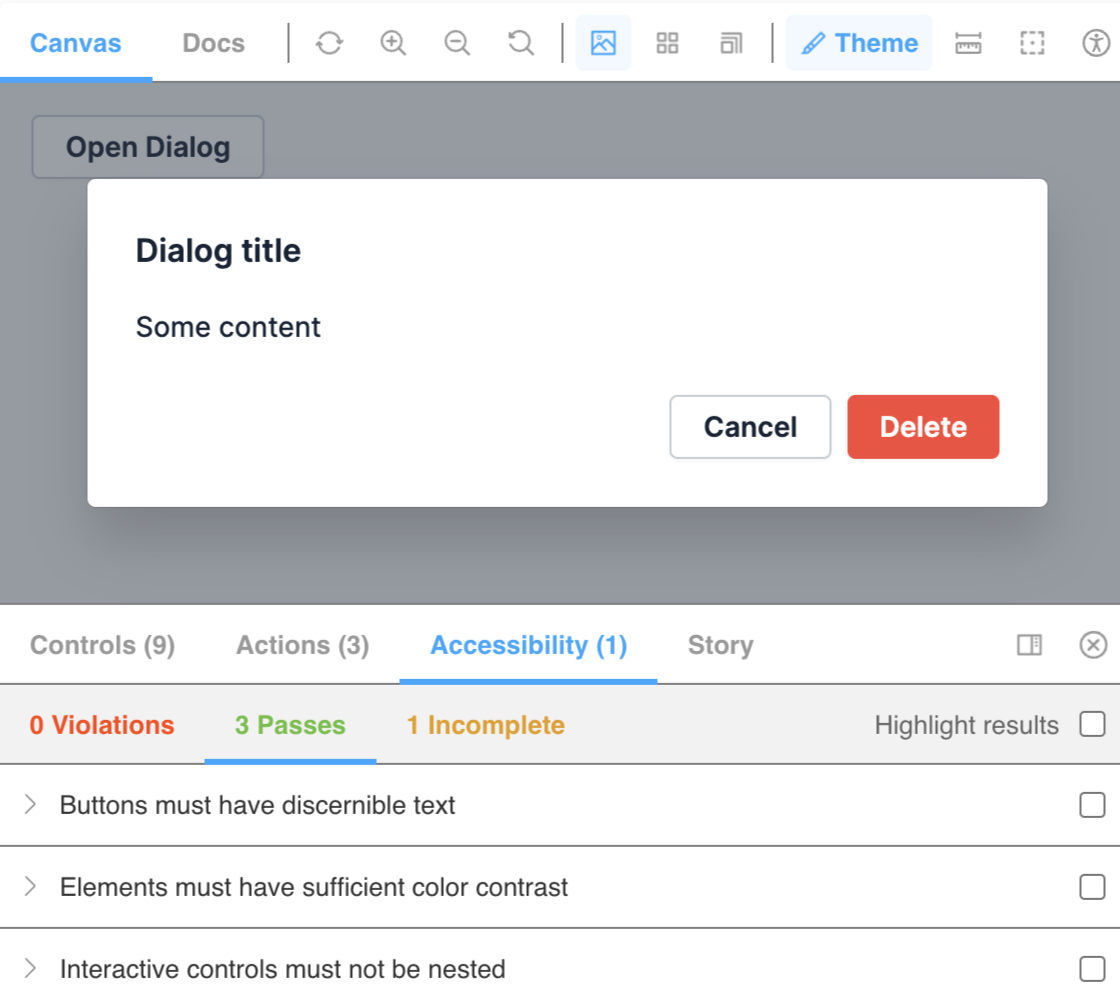
\includegraphics[width=\textwidth]{img/sb-button-trigger-open.png}
	\caption{Example after clicking the button and revealing the actual component.}
	\label{fig:sb-button-trigger-2}
	\end{subfigure}
\caption{Storybook example for Dialog component using button trigger}
\label{fig:sb-button-trigger}
\end{figure}

Looking at all the fails and passes gives an overview of how many tests were run for each component. Out of 53 components, only 2 (4\%) did not get checked by addon-a11y at all, but after validating the results this number changes to 20 (38\%). This includes components that become visible only when triggered by another element, like modals and popups that are currently displayed with a button as a trigger in the Storybook examples (see Figure \ref{fig:sb-button-trigger}). These components are seen in Figure \ref{fig:audit-passed} starting from \textit{VideoOverlay} and ending with \textit{Coachmark} - 11 overall.

The rest of the components that did not get tested by the addon included very simple components for spacing and visuals. These need further testing when they are being used in context to make sure that the visual info they are conveying is also included in text form. The results from manual testing did not reveal any further issues for 6 of these components. The components that have a trigger button in the example had the most additional issues. This is expected as due to the limitation of the examples the correct component was not evaluated by the tool.

\begin{figure}[ht]
	\centering
	\begin{subfigure}{0.4\textwidth}
	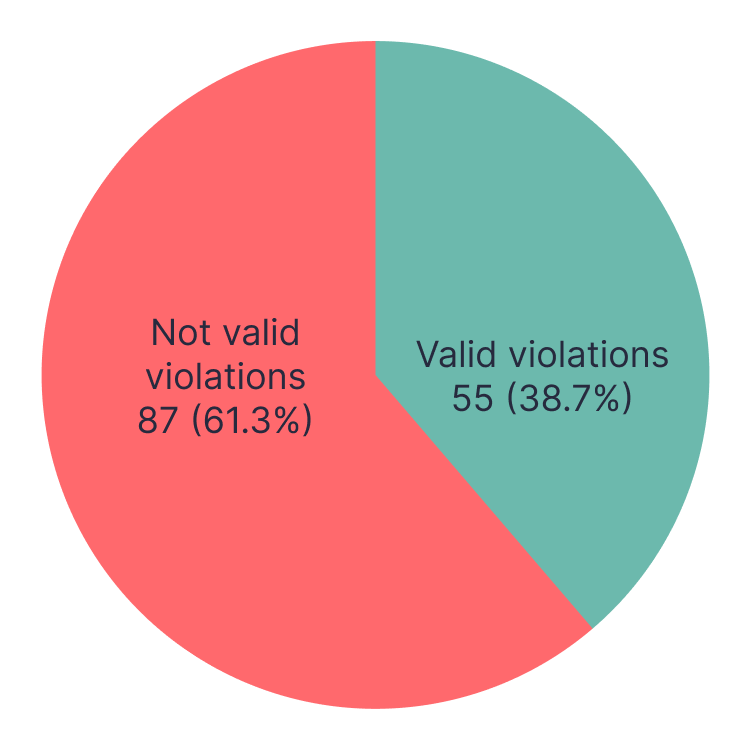
\includegraphics[width=\textwidth]{img/failed-tests.png}
	\caption{How many of the detected violations are valid?}
	\label{fig:checks-validity-failed}
	\end{subfigure}
	\hspace{0.05\textwidth}
	\begin{subfigure}{0.4\textwidth}
	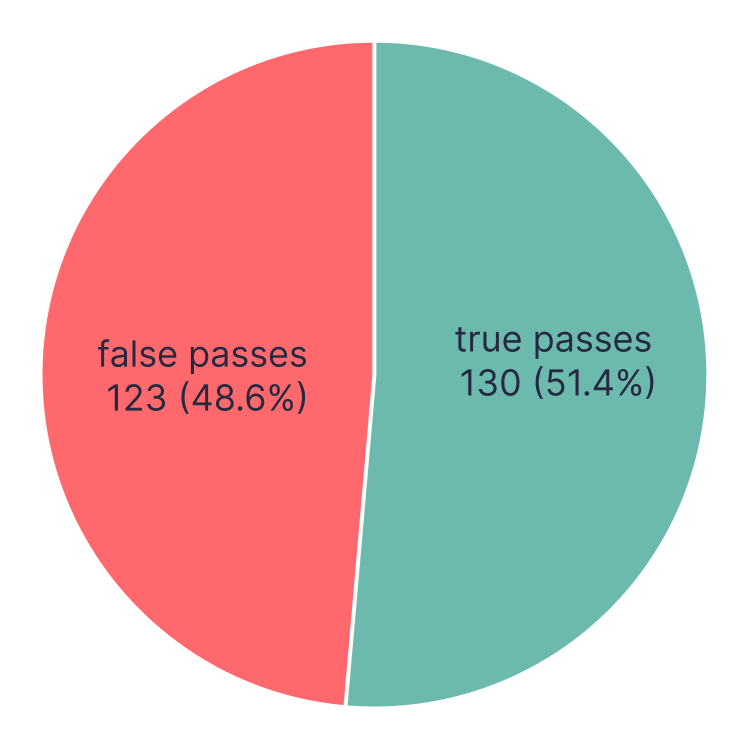
\includegraphics[width=\textwidth]{img/passed-tests.png}
	\caption{How many of the checks passed are valid?}
	\label{fig:checks-validity-passed}
	\end{subfigure}
	\hspace{0.05\textwidth}
	\begin{subfigure}{0.4\textwidth}
	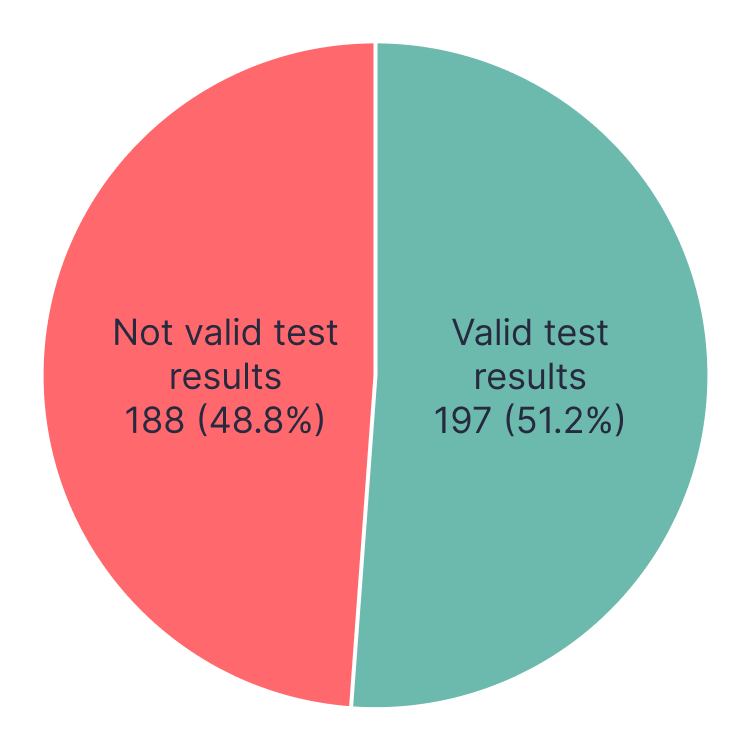
\includegraphics[width=\textwidth]{img/all-test-results.png}
	\caption{How many of all tests are valid?}
	\label{fig:checks-validity-all}
	\end{subfigure}
\caption{Valididty of tests performed by addon-a11y}
\label{fig:checks-validity}
\end{figure}

Analyzing the validity of checks performed by addon-a11y further shows that from all passes and fails together a bit more than half are valid while 68\% of detected violations are correct and 51\% of passed checks were confirmed to be relevant (see Figure \ref{fig:checks-validity}).

\review{Mari-Ell: Do you have a solution on how to get them tested as well? Somehow display them without the need of the trigger? - Test out play functions with Storybook 7 and the built-in test runner.}

\begin{figure}[ht]
	\begin{subfigure}{0.45\textwidth}
	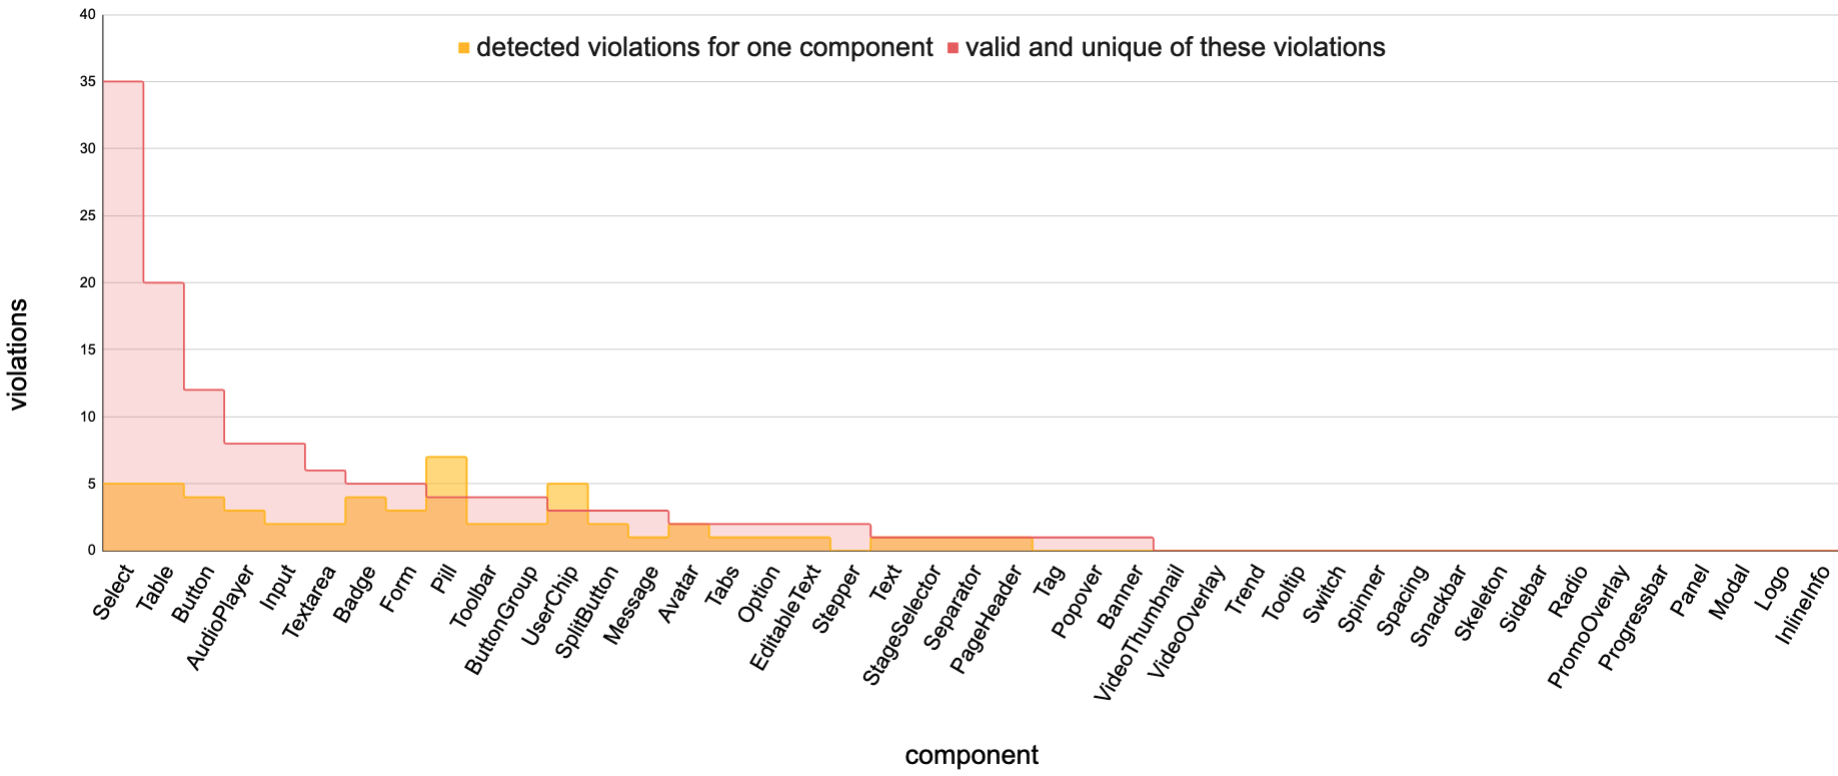
\includegraphics[height=0.9\textheight]{img/audit-failed.png}
	\caption{All violations reported by addon-a11y and how many of them are valid.}
	\label{fig:audit-failed}
	\end{subfigure}
	\hspace{0.05\textwidth}
	\begin{subfigure}{0.45\textwidth}
	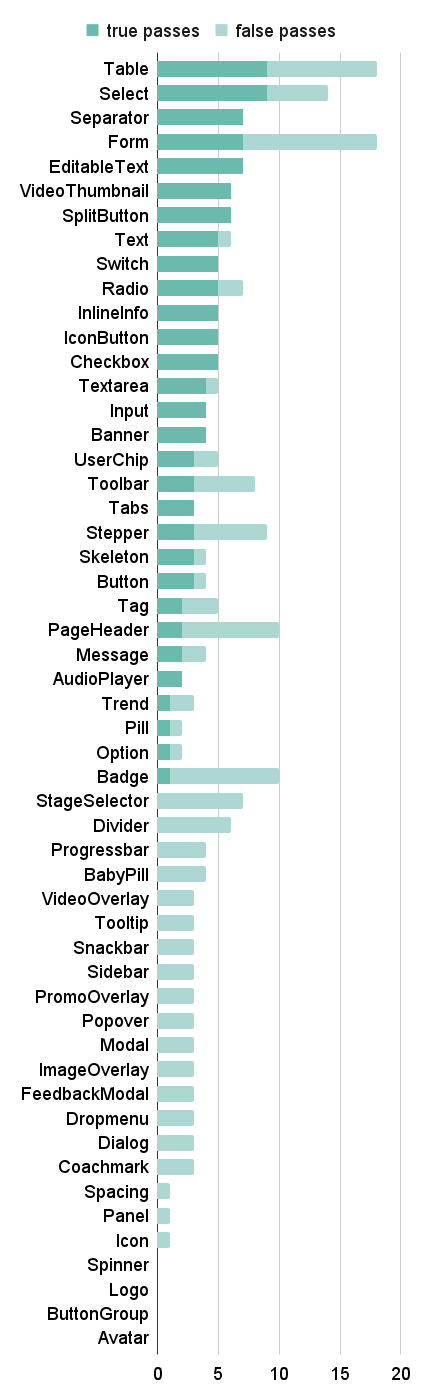
\includegraphics[height=0.9\textheight]{img/audit-passed.png}
	\caption{All passed checks reported by addon-a11y and how many of them are valid.}
	\label{fig:audit-passed}
	\end{subfigure}
\caption{All issues checked by addon-a11y}
\label{fig:audit-passed-failed}
\end{figure}

\end{document}